\chapter{Conclusiones}

\section{Cumplimiento de los objetivos}

El objetivo principal del proyecto era crear un vehículo a escala que
pueda ser controlado de manera remota por el usuario, se pudo comprobar
la viabilidad tanto en términos de hardware como de software de los
objetivos planteados desde un principio. Permitiendo, de esta manera, el
desarrollo total del proyecto en tiempo y forma.

A su vez, se dividió el proyecto en 4 partes principales:

\begin{enumerate}
\def\labelenumi{\arabic{enumi}.}
\tightlist
\item
  Estructura física del vehículo
\end{enumerate}

La estructura del vehículo fue realizada con la carcaza de una lectora
de CD (ver foto \ref{fig:agujero-caja}). La misma fue modificada para poder colocar los 4 motores, la
EDU-CIAA junto con el poncho y las pilas de litio.

Para una mejor apariencia física, se optó por remover la tapa superior
de la carcaza. De esta manera, quedan a simple vista todos los
componentes que conforman el vehículo.

La estructura demostró ser lo suficientemente rígida y ligera para
soportar todos los componentes de hardware, y a su vez, permiter que los
motores puedan transportarla sin la necesidad de una potencia excesiva.

\begin{enumerate}
\def\labelenumi{\arabic{enumi}.}
\setcounter{enumi}{1}
\tightlist
\item
  Control de motores
\end{enumerate}

El control de los motores del vehículo se realizó a través del integrado
L293D, el cual cuenta con dos puente H completos. Estos están ubicados
sobre el poncho, distribuidos de manera que el conexionado permita que
con un integrado se controle el motor delantero y trasero de un lateral
del vehículo.

Cada motor permite el movimiento en ambos sentidos de giro, de manera
que el vehículo cumple con los objetivos de avanzar, rotar y retroceder.

\begin{enumerate}
\def\labelenumi{\arabic{enumi}.}
\setcounter{enumi}{2}
\tightlist
\item
  Control remoto
\end{enumerate}

El usuario puede controlar el vehículo de manera remota utilizando el
módulo HM-10, el cual funciona mediante el protocolo bluetooth.

Se optó por utilizar una aplicación de android ya implementada
``BLEJoystick'', disponible en Google Play Store, siendo esta muy simple
y sencilla de utilizar. De esta manera, se cumplió con el objetivo de
poder manejar el vehículo desde una distancia de hasta aproximadamente
20 metros.

\begin{enumerate}
\def\labelenumi{\arabic{enumi}.}
\setcounter{enumi}{3}
\tightlist
\item
  Medición de sensores y respuesta en consecuencia
\end{enumerate}

Con el fin de detectar objetos/obstáculos delante del vehículo, se
cuenta con un sensor de proximidad ultrasónico HC-SR04, ubicado en el
frente del poncho.

Luego de realizar algunas pruebas, se observó que la distancia para
bloquear el avance del vehículo debía ser configurada con algunos
centímetros extras de margen, debido al tiempo de respuesta del sensor.
De esta manera, se fijó una distancia máxima de 30cm, con un ángulo de
visión de 15°, cumpliendo con el objetivo de bloquear el avance del
vehículo justo antes de impactar con cualquier objeto.

A su vez, se agregó un buzzer con el objetivo de indicar el evento de
colisión mediante sonido, generando una alerta cada vez que se detecta
un obstáculo antes de realizar el bloqueo total del vehículo.

No ha sido implementado el objetivo secundario del sensor de luminosidad
LDR, debido a la demanda de tiempo de dicha tarea y a la complejidad del
diseño del poncho.

\section{Cumplimiento de Requerimientos}

\subsection{Requerimientos Funcionales}

\subsubsection{Requerimientos de Software}

\paragraph{Control de Motores}

\begin{enumerate}
\def\labelenumi{\arabic{enumi}.}
\item
  El sistema debe accionar 4 motores individualmente, permitiendo girar
  en ambas direcciones.

  Se cumplió con el objetivo parcialmente. Dado que el pin \emph{enable}
  de los L293D es compartido por todos los motores, por lo que se
  obtienen las siguientes características:

  \begin{itemize}
  \tightlist
  \item
    Todas las ruedas se accionan en simultaneo, es decir, giran todas o
    no gira ninguna.\\
  \item
    La velocidad de todas las ruedas puede controlarse de igual manera.
  \item
    Individualmente puede controlarse: dirección de giro y frenado
    rápido.
  \end{itemize}
\item
  El sistema debe accionar motores en conjunto, permitiendo avanzar,
  retroceder y girar.

  Se cumplió completamente con el objetivo, ya que se puede:

	\begin{itemize}
	\tightlist
	\item
	  Avanzar si toda las ruedas giran hacia adelante.
	\item
	  Retroceder si todas las ruedas giran hacia atrás
	\item
	  Girar para ambos lados, si un par lateral trata de avanzar y el otro
	  par retroceder. Como podemos ver a continuación:
	\end{itemize}

\end{enumerate}

\begin{figure}[H]
\centering
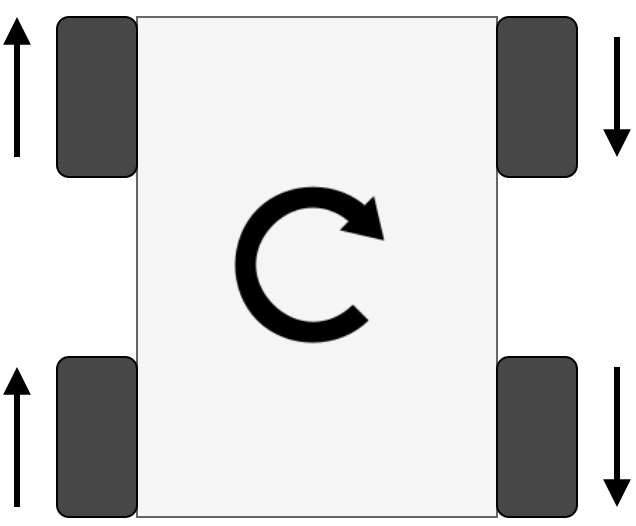
\includegraphics[width=0.4\linewidth]{informe_4/diagrama_giro.png}
\caption{Dirección de giro}
\end{figure}

\begin{enumerate}
\def\labelenumi{\arabic{enumi}.}
\setcounter{enumi}{2}
\item
  El sistema debe permitir el bloqueo de movimiento en una dirección
  (por ejemplo debido a un obstáulo detectado por el sensor de
  proximidad).

  Se cumplió parcialmente con el objetivo, ya que se puede bloquear solo
  el movimiento hacia adelante. Esto puede verse en el código:

\begin{lstlisting}
//bloquea el avance del vehiculo
void bloquear() {
   avance_bloqueado = TRUE;
}

...

void actualizar_desplazamiento() {

    switch (estado_auto) {

     //si el estado es adelante, todos los motores giran en un mismo sentido
     case ADELANTE:
         //El avance puede ser bloqueado por el detector de colisiones. En ese caso, se vuelve a actualizar el estado del vehiculo
         if (avance_bloqueado){
             estado_auto = FRENADO;
         }else{
             set_motor(M_DELANTERO_DER, M_MOV_ADELANTE, velocidad_avance);
             set_motor(M_DELANTERO_IZQ, M_MOV_ADELANTE, velocidad_avance);
             set_motor(M_TRASERO_DER, M_MOV_ADELANTE, velocidad_avance);
             set_motor(M_TRASERO_IZQ, M_MOV_ADELANTE, velocidad_avance);
         }
         break;

        ...
     }
\end{lstlisting}
\item
  OPT El sistema debe indicar mediante una serie de LEDs el estado de
  movimiento del vehículo.

No se cumplió con el objetivo opcional, ya que se buscó simplificar el
diseño del poncho.
\end{enumerate}

\paragraph{Control Remoto}

\begin{enumerate}
\def\labelenumi{\arabic{enumi}.}
\item
  El sistema debe establecer una conexión bluetooth con el sistema de
  control remoto.

  Se cumplió con el objetivo, utilizando un módulo Bluetooth HM-10
  provisto por la cátedra.
\item
  El sistema debe leer las indicaciones del control remoto y ejecutar
  las acciones correspondientes.

  Se cumplió con el objetivo, utilizando como control remoto una
  aplicación de celular, cuyo funcionamiento ya fue detallado con
  anterioridad.
\item
  El sistema debe indicar mediante un LED el estado de la conexión
  bluetooth.

  Se utilizó el LED que viene incluído en el módulo HM-10, que indica
  con una luz parpadeante si recibe alimentación, y una luz constante si
  se realizó la conexión.
\end{enumerate}

\paragraph{OPT Medición Sensores}

\begin{enumerate}
\def\labelenumi{\arabic{enumi}.}
\item
  Ante ausencia de luz externa, se deben encender las luces del vehículo

  No se cumplió con el objetivo, por demanda de tiempo y para
  simplificar el diseño del poncho.
\item
  Ante la presencia de obstáculos, se debe frenar el desplazamiento en
  esa dirección.

  Se cumplió con el objetivo, utilizando un sensor de proximidad
  ultrasónica, HC-SR04. Al utilizar un único sensor, con ángulo de
  visión de 15°, el vehículo solo frena el desplazamiento hacia
  adelante.
\end{enumerate}

\subsubsection{Requerimientos de Hardware}

\paragraph{Control de Motores}

\begin{enumerate}
\def\labelenumi{\arabic{enumi}.}
\item
  El vehículo debe utilizar puentes H para motores de corriente
  continua.

  Se cumplió con el objetivo, utilizando dos integrados L293D, dónde
  cada uno posee dos puentes H.
\item
  OPT El vehículo debe indicar con un LED para cada motor si este está
  en movimiento.

  No se cumplió con el objetivo, para simplificar el diseño del poncho.
\end{enumerate}

\paragraph{Baterías y cargador}

\begin{enumerate}
\def\labelenumi{\arabic{enumi}.}
\item
  El vehículo debe utilizar baterías de Litio para lograr la autonomía
  del vehículo

  Se cumplió con el objetivo, utilizando dos baterías de Litio en serie
  obteniendo una tensión de alimentación de aproximadamente 8V.
\item
  El vehículo debe indicar mediante un LED cuando haya baja tensión

  No se cumplió con el objetivo, no se pudo encontrar una manera
  sencilla de implementarlo.
\item
  El vehículo debe permitir cargar las baterías mediante un puerto USB.

  No se cumplió con el objetivo, ya que cargar el dispostivo con todos
  los componentes conectados podría generar problemas eléctricos.
\end{enumerate}

\paragraph{Componentes}

\begin{enumerate}
\def\labelenumi{\arabic{enumi}.}
\item
  Se debe contar con una llave de encendido/apagado y un LED que
  determine su estado.

  Se cumplió con el objetivo, se cuenta con una llave y varios LEDs que
  indican estado, ya que hay LEDs de alimentación en el Poncho, en la
  EDU-CIAA y en el módulo Bluetooth.
\item
  OPT El sistema debe poseer un buzzer para indicar eventos o fallas

  Se cumplió con el objetivo, el buzzer cumple dos funciones; notificar
  la presencia de obstáculos antes de bloquear el avance e indicar si el
  vehículo está retrocediendo.
\end{enumerate}

\subsection{Requerimientos No Funcionales}

\begin{itemize}
\tightlist
\item
  Utilizacion de la placa de desarrollo EDU-CIAA.
\item
  Estructura sólida y liviana, donde se colocan los motores y la
  EDU-CIAA.
\item
  El conexionado a los motores debe ser a través de borneras para poder
  cambiar la estructura.
\item
  Programación en lenguaje C.
\item
  Desarrollo de PCB en formato de poncho.
\item
  Mecanismo de control simple.
\item
  El sistema debe manejar respuestas en tiempo real.
\item
  Fecha de finalización y entrega del proyecto el día 16/12.
\end{itemize}

Se cumplieron todos los requerimientos no funcionales en tiempo y forma.

\subsection{Evaluación}

El grado de cumplimiento de los objetivos, en general, fue altamente
positivo. Los requerimientos funcionales que no se llevaron a cabo
fueron los de menor prioridad, la mayoría relacionados al hardware,
debido a que implicaban un costo de implementación muy alto para obtener
una funcionalidad muy reducida. Por ejemplo, el caso de colocar un led
que indique el estado de cada motor, lo cual costaría 4 pines GPIO, más
toda su interconexión, aumentando aún más la complejidad del poncho.

El principal cambio realizado fue el uso de una placa doble faz, por dos
motivos:

\begin{enumerate}
\def\labelenumi{\arabic{enumi}.}
\item
  Obtener un plano de tierra para disipar el calor producido por los
  integrados L293D.
\item
  Facilitar la conexión a tierra de los componentes, junto con el uso de
  puentes.
\end{enumerate}

Otro cambio fue el uso de una sola fuente step-down. En un principio la
alimentación iba a consistir de dos pilas de litio en paralelo, las
cuales entregarían aproximadamente 4v, y creíamos que sería necesario
utilizar dos conversores; un conversor step-up para alimentar los L293D
con 8v, y un conversor step-down para alimentar la EDU-CIAA con 3.3v.

Una vez estudiada mejor la arquitectura de la EDU-CIAA, observamos que
se alimentaba con 5v, y que internamente tiene un conversor a 3.3v para
aquellos puertos o componentes que necesiten de dicha tensión. Por este
motivo, cambiamos las pilas de paralelo a serie para obtener 8v que
alimentan directamente a los L293D, y utilizamos una fuente step-down
para alimentar la EDU-CIAA con 5v a través del conector Molex para
alimentación externa.

Un error que cometimos fue implementar mal la huella del conversor
step-down, la cual quedó completamente espejada, por lo que hubo que
colocarla sobre pines, y la tierra soldarla sobre el plano en lugar de
atravezando la placa.

\section{Actividad de los integrantes}

\begin{longtable}[]{@{}lll@{}}
\toprule
\begin{minipage}[b]{0.17\columnwidth}\raggedright
Tarea\strut
\end{minipage} & \begin{minipage}[b]{0.64\columnwidth}\raggedright
Descripción\strut
\end{minipage} & \begin{minipage}[b]{0.10\columnwidth}\raggedright
Tiempo\strut
\end{minipage}\tabularnewline
\midrule
\endhead
\begin{minipage}[t]{0.17\columnwidth}\raggedright
Compra de componentes\strut
\end{minipage} & \begin{minipage}[t]{0.64\columnwidth}\raggedright
Se obtuvieron los componentes electrónicos principales, los puentes H
(L293D) no se consiguieron individualmente por lo que se compró un
shield de Arduino que posee 2. Todos los componentes fueron comprados en
La Plata salvo las ruedas y motores. Componentes que requerían valores
precisos como resistencias y capacitores se fueron comprando a medida
que se concretaba el diseño.\strut
\end{minipage} & \begin{minipage}[t]{0.10\columnwidth}\raggedright
3 Horas\strut
\end{minipage}\tabularnewline
\begin{minipage}[t]{0.17\columnwidth}\raggedright
Estudio BT\strut
\end{minipage} & \begin{minipage}[t]{0.64\columnwidth}\raggedright
Mediante el uso de un módulo HM-10, el programa Hércules, la sAPI y un
aplicación para Android, se estudió el funcionamiento de la comunicación
Bluetooth. Se pudo concluir lo descripto en la sección de Software,
Bluetooth.\strut
\end{minipage} & \begin{minipage}[t]{0.10\columnwidth}\raggedright
8 Horas\strut
\end{minipage}\tabularnewline
\begin{minipage}[t]{0.17\columnwidth}\raggedright
Arquitectura de Software\strut
\end{minipage} & \begin{minipage}[t]{0.64\columnwidth}\raggedright
Se diseño la estructura principal del programa, como se describió en la
sección de software\strut
\end{minipage} & \begin{minipage}[t]{0.10\columnwidth}\raggedright
4 Horas\strut
\end{minipage}\tabularnewline
\begin{minipage}[t]{0.17\columnwidth}\raggedright
Estudio L293D\strut
\end{minipage} & \begin{minipage}[t]{0.64\columnwidth}\raggedright
Leyendo las datasheets del L293D y con recomendaciones de la cátedra, se
llegó a un diseño para la PCB que cumplía con los requisitos eléctricos
y térmicos. Además aquí también se incluye la investigación del módulo
PWM de la EDU-CIAA, para poder controlar la potencia de los
motores\strut
\end{minipage} & \begin{minipage}[t]{0.10\columnwidth}\raggedright
8 horas\strut
\end{minipage}\tabularnewline
\begin{minipage}[t]{0.17\columnwidth}\raggedright
Prototipo L293D\strut
\end{minipage} & \begin{minipage}[t]{0.64\columnwidth}\raggedright
Se utilizó un Arduino y el Shield mencionado para probar algunos motores
y el funcionamiento de los puentes H\strut
\end{minipage} & \begin{minipage}[t]{0.10\columnwidth}\raggedright
8 horas\strut
\end{minipage}\tabularnewline
\begin{minipage}[t]{0.17\columnwidth}\raggedright
Estudio de sensores\strut
\end{minipage} & \begin{minipage}[t]{0.64\columnwidth}\raggedright
Se investigó principalmente el funcionamiento del sensor de proximidad
HC-SR04\strut
\end{minipage} & \begin{minipage}[t]{0.10\columnwidth}\raggedright
4 horas\strut
\end{minipage}\tabularnewline
\begin{minipage}[t]{0.17\columnwidth}\raggedright
Estudio de batería\strut
\end{minipage} & \begin{minipage}[t]{0.64\columnwidth}\raggedright
Se vieron diferences opciones para la implementación de las baterías, la
caída de tensión en el L293D, tensión de las pilas de litio\strut
\end{minipage} & \begin{minipage}[t]{0.10\columnwidth}\raggedright
2 horas\strut
\end{minipage}\tabularnewline
\begin{minipage}[t]{0.17\columnwidth}\raggedright
Desarrollo de Software prioritario\strut
\end{minipage} & \begin{minipage}[t]{0.64\columnwidth}\raggedright
Se implementaron las partes más importantes del programa, el control de
motores y la comunicación Bluetooth\strut
\end{minipage} & \begin{minipage}[t]{0.10\columnwidth}\raggedright
8 horas\strut
\end{minipage}\tabularnewline
\begin{minipage}[t]{0.17\columnwidth}\raggedright
Estructura\strut
\end{minipage} & \begin{minipage}[t]{0.64\columnwidth}\raggedright
Se dejó para el final para centrarnos en la investigación y desarrollo
del poncho\strut
\end{minipage} & \begin{minipage}[t]{0.10\columnwidth}\raggedright
4 horas\strut
\end{minipage}\tabularnewline
\begin{minipage}[t]{0.17\columnwidth}\raggedright
Prototipo de Estructura\strut
\end{minipage} & \begin{minipage}[t]{0.64\columnwidth}\raggedright
El prototipo fue una precaria caja de zapatos, como se puede observar en
las fotos\strut
\end{minipage} & \begin{minipage}[t]{0.10\columnwidth}\raggedright
4 horas\strut
\end{minipage}\tabularnewline
\begin{minipage}[t]{0.17\columnwidth}\raggedright
Diseño de PCB\strut
\end{minipage} & \begin{minipage}[t]{0.64\columnwidth}\raggedright
El diseño de la PCB fue evolucionando constantemente, la estructura y
disposición de los componentes se mantuvo pero se fueron optimizando las
pistas.\strut
\end{minipage} & \begin{minipage}[t]{0.10\columnwidth}\raggedright
16 horas\strut
\end{minipage}\tabularnewline
\begin{minipage}[t]{0.17\columnwidth}\raggedright
Fabricación de PCB\strut
\end{minipage} & \begin{minipage}[t]{0.64\columnwidth}\raggedright
La PCB se fabricó en el ATEI con ayuda de Alejandro\strut
\end{minipage} & \begin{minipage}[t]{0.10\columnwidth}\raggedright
6 horas\strut
\end{minipage}\tabularnewline
\begin{minipage}[t]{0.17\columnwidth}\raggedright
Desarrollo de software secundario\strut
\end{minipage} & \begin{minipage}[t]{0.64\columnwidth}\raggedright
No se cumplió con el cronograma original, y se desarrollo los últimos
días\strut
\end{minipage} & \begin{minipage}[t]{0.10\columnwidth}\raggedright
6 horas\strut
\end{minipage}\tabularnewline
\begin{minipage}[t]{0.17\columnwidth}\raggedright
Montaje\strut
\end{minipage} & \begin{minipage}[t]{0.64\columnwidth}\raggedright
Se soldaron los componentes, se colocaron los motores, tornillos de
montaje, y porta pilas\strut
\end{minipage} & \begin{minipage}[t]{0.10\columnwidth}\raggedright
6 horas\strut
\end{minipage}\tabularnewline
\begin{minipage}[t]{0.17\columnwidth}\raggedright
Elección de baterías\strut
\end{minipage} & \begin{minipage}[t]{0.64\columnwidth}\raggedright
Dado el tamaño solo cabían dos pilas, las necesarias para llegar
8v.\strut
\end{minipage} & \begin{minipage}[t]{0.10\columnwidth}\raggedright
2 minutos\strut
\end{minipage}\tabularnewline
\begin{minipage}[t]{0.17\columnwidth}\raggedright
Calibración de Motores\strut
\end{minipage} & \begin{minipage}[t]{0.64\columnwidth}\raggedright
Se reguló la velocidad y se verificó que el mapeo de software coincida
con la implementación en hardware\strut
\end{minipage} & \begin{minipage}[t]{0.10\columnwidth}\raggedright
30 minutos\strut
\end{minipage}\tabularnewline
\begin{minipage}[t]{0.17\columnwidth}\raggedright
Validación\strut
\end{minipage} & \begin{minipage}[t]{0.64\columnwidth}\raggedright
Se verificó que el poncho y el software funciona correctamente y de
acuerdo a lo especificado. Hubo que reprogramar diveros sectores, como
el sensor de proximidad, que no actuaban acorde a lo especificado\strut
\end{minipage} & \begin{minipage}[t]{0.10\columnwidth}\raggedright
12 horas\strut
\end{minipage}\tabularnewline
\bottomrule
\end{longtable}

\section{Presupuesto}

\begin{longtable}[]{@{}ll@{}}
\toprule
Producto & Precio\tabularnewline
\midrule
\endhead
Shield motor driver arduino & \$ 350\tabularnewline
Ruedas con caja reductora y motores & \$ 1200\tabularnewline
Porta pilas de litio & \$ 150\tabularnewline
Placa virgen 10x15 doble faz & \$ 180\tabularnewline
Mini switch & \$ 45\tabularnewline
HC-SR04 & \$ 170\tabularnewline
Tira de 2x40 pines macho & \$ 80\tabularnewline
Step Down mini 360 & \$ 150\tabularnewline
Buzzer & \$ 30\tabularnewline
Resistencias/capacitores/leds/varios & \$ 200\tabularnewline
Transistor 2n7000 & \$ 20\tabularnewline
Hoja A4 papel fotográfico & \$ 20\tabularnewline
Horas de ingeniería (400hs.) & \$ 72000\tabularnewline
Total & \$ 74595\tabularnewline
\bottomrule
\end{longtable}
